% ============================================================================
% CAISc 2026 — Verifiable Track submission (ANONYMIZED / double-blind)
% Problem: Connected Maximum-Density Still Life (Conway's Game of Life)
%
% COMPILE: pdflatex (US Letter). Requires caisc_2026.sty in the same directory.
% Default \usepackage{caisc_2026} (no options) = anonymized + line numbers.
%   DO NOT add [final] or [preprint] for the blind submission.
%
% TODO before submission:
%   [T1] DONE -- n=16..21 filled as best-found; n=31/32 excluded (embed-only,
%        not a meaningful bound).
%   [T2] RESOLVED -- independent ASP cross-check did not terminate in budget;
%        n=10/11 rest on the CP-SAT certificate (stated in text and limitations).
%   [T3] Paste the exact problem "Cite This Problem" string into \bibitem{problem}.
%   [T4] Confirm metadata for \bibitem{aspcomp2013} and \bibitem{satlution}.
%   [T5] DONE -- Figure 1 renders the proven-optimal n=8 witness.
%   [T6] Authors and acknowledgments are added ONLY in the
%        camera-ready [final] version. Keep them OUT of this blind submission.
%   [T7 DONE] AI Involvement letter grades / iteration levels confirmed by the author
%        reflect his view of the human/AI split (drafted honestly from the log).
% ============================================================================

\PassOptionsToPackage{numbers,compress}{natbib}
\documentclass{article}

\usepackage{caisc_2026}      % ready for submission (anonymized + line numbers)

\usepackage[utf8]{inputenc}
\usepackage[T1]{fontenc}
\usepackage{hyperref}
\usepackage{url}
\usepackage{booktabs}
\usepackage{amsfonts}
\usepackage{amsmath}
\usepackage{amssymb}
\usepackage{amsthm}
\usepackage{nicefrac}
\usepackage{microtype}
\usepackage{xcolor}
\usepackage{graphicx}
\usepackage{tikz}

\newcommand{\copt}{\textsc{c\textendash opt}}
\newtheorem{proposition}{Proposition}

\title{Connected Maximum-Density Still Lifes in Conway's Game of Life\\via a Verifier-Grounded Agentic Loop}

% Authors are intentionally omitted for double-blind review (the style file
% renders "Anonymous Author(s)" in submission mode). Real authorship is added
% only in the camera-ready [final] version. See [T6].
\author{%
  Anonymous Author(s) \\
  Affiliation \\
  Address \\
  \texttt{email} \\
}

\begin{document}

\maketitle

\begin{abstract}
We study the connected maximum-density still life problem in Conway's Game of Life---maximizing the number of live cells in a stable, $8$-connected pattern inside an $n\times n$ box---a problem from the CAISc 2026 verifiable-problems list. The unconstrained variant is completely solved, but to the best of our knowledge no per-$n$ table of \emph{connected} optima has previously been published. We attack the problem with a verifier-grounded agentic loop: a large language model orchestrates a grader-faithful deterministic verifier, two independent exact engines (a CP-SAT model cross-checked under two independent connectivity encodings, single-commodity flow and spanning tree, and an independently reproduced answer-set-programming encoding), and a stochastic proposer, re-routing among them based on observed solver behavior. The verifier validates every claimed pattern, so no reported result rests on solver trust alone. We contribute the first per-$n$ connected table for the small boxes: connected optima \emph{proven} for $n\in\{8,9,10,11\}$ (respectively $32$, $43$, $53$, and $63$ live cells), and verifier-validated best-found values with two-sided bounds for $n\in\{13,15\}$, and verifier-validated best-found patterns for $16\le n\le 21$ from a budgeted constraint-solver heuristic. We also report three methodological findings: a sandwich ``ceiling-matching'' argument that proves optimality without exhaustive search whenever a connected witness meets the proven unconstrained optimum; evidence that the CP-SAT flow encoding outperforms the ASP reachability encoding on proof closure for $n\ge 10$; and a diagnosis of why naive verify-or-reject simulated annealing fails on this problem. All witness patterns and the verifier are released as machine-checkable artifacts.
\end{abstract}

\section{Introduction}
\label{sec:intro}

Conway's Game of Life is a two-state cellular automaton on the square grid in which a live cell survives with two or three live neighbors and a dead cell is born with exactly three. A \emph{still life} is a pattern fixed under this rule. The maximum-density still life problem---how many live cells fit in an $n\times n$ box without instability---is a classic constraint-optimization benchmark and was completely solved by Chu and Stuckey~\citep{chu2012}, whose values coincide with OEIS sequence A055397~\citep{oeis}. Those optima are \emph{pseudo} still lifes: they need not be connected, and for several box sizes the densest stable pattern is in fact a regular array of disjoint blocks.

The \emph{connected} variant adds a single global constraint---all live cells must form one island under $8$-adjacency---and is the subject of this paper and of the corresponding CAISc 2026 verifiable problem~\citep{problem}. Connectivity changes the optimization in a way that is poorly documented: it appears only as a benchmark in the ASP Competition~\citep{aspcomp2013}, which measured solver performance rather than publishing per-$n$ optima, and to the best of our knowledge---after searching the standard still-life references, community censuses, and competition reports---no maintained per-$n$ table of connected optima or best-known values exists. This gap is the opportunity.

CAISc rewards the AI-driven methodology as much as the combinatorial result. Our primary contribution is therefore an \emph{agentic discovery loop} and its application, not merely a list of patterns:

\begin{itemize}
\item \textbf{A verifier-grounded agentic architecture.} A large language model orchestrates a grader-faithful deterministic verifier, two independent exact engines (CP-SAT with a single-commodity-flow connectivity encoding; a reproduced ASP reachability encoding), and a stochastic proposer. The deterministic verifier is foundational: every reported pattern is re-checked against it, so validity never depends on trusting a solver or the agent.
\item \textbf{The first per-$n$ connected table for small boxes.} We prove the connected optimum for $n\in\{8,9,10,11\}$ and give verifier-validated best-found values with two-sided bounds for $n\in\{13,15\}$; for $16\le n\le 21$ we report verifier-validated best-found patterns.
\item \textbf{Methodological findings.} (i) A ``ceiling-matching'' sandwich argument (Proposition~\ref{prop:ceiling}) that proves optimality without exhaustive search whenever a connected witness meets the proven unconstrained ceiling. (ii) Evidence that, on the connectivity-augmented Life encoding, a CP-SAT flow formulation closes proofs that an ASP reachability formulation cannot for $n\ge 10$. (iii) A diagnosis of why naive verify-or-reject simulated annealing makes no valid progress on this problem, which is itself an explanation for why the literature reaches for exact and hybrid methods.
\end{itemize}

\paragraph{Claims and scope.} We claim proven optimality only for $n\in\{8,9,10,11\}$; all other reported values are explicitly labeled best-found, with bounds where available. Every claimed pattern is validated by the released verifier in the official submission format. We make no claim of having found the connected optimum for $n\ge 13$.

\section{Problem definition and background}
\label{sec:problem}

\paragraph{Definition.} Fix a box size $n$. A configuration is an assignment of $\{0,1\}$ to the cells of an $n\times n$ grid. Writing $N(i,j)$ for the number of live cells among the eight Moore neighbors of $(i,j)$, the configuration is a \emph{connected still life} iff: (1) every live cell $(i,j)$ has $N(i,j)\in\{2,3\}$ (stability); (2) no dead cell has $N(i,j)=3$, where this birth condition is checked for every cell of the box \emph{and} of its one-cell exterior ring (no births); and (3) the live cells form a single $8$-connected component. The objective is to maximize the number of live cells. We denote the connected optimum by $\copt(n)$ and the unconstrained optimum by $a(n)=$ A055397$(n)$. Permitted box sizes are $n\in\{8,9,10,11,13,15,16,17,19,20,21,31,32\}$~\citep{problem}.

\paragraph{The ceiling.} Because every connected still life is a still life, restricting to connected patterns can only shrink the feasible set, so $\copt(n)\le a(n)$ for all $n$. The values $a(n)$ are proven optimal~\citep{chu2012} and serve as our upper bounds throughout (Table~\ref{tab:main}). They are attained by possibly-disconnected patterns; for box sizes of the form $3k-1$ (including $n=8$ and $n=11$ among our set) the densest stable configuration is a disjoint block array, so a strict gap $\copt(n)<a(n)$ is expected there. Elkies~\citep{elkies1998} proved that the infinite-lattice still-life density is at most $\nicefrac{1}{2}$; finite boxes can exceed this, and our connected densities sit just above $50\%$, consistent with that bound.

\paragraph{Related work.} Exact approaches to the unconstrained problem include hybrid integer/constraint programming~\citep{bosch2004}, variable (bucket) elimination~\citep{larrosa2005}, dedicated constraint models~\citep{chu2010}, and the lazy-clause-generation solution that closed the problem~\citep{chu2012}; memetic/exact hybrids gave strong large-instance results~\citep{gallardo2009}. Enforcing connectivity in combinatorial models is itself well studied---single- and multi-commodity flow, spanning-tree, and lazy separator-cut formulations are standard tools. Methodologically, our loop follows recent work pairing generative models with deterministic evaluators for discovery: program search with an evaluator~\citep{funsearch}, evolutionary coding agents~\citep{alphaevolve}, and solver-evolution under strict verification~\citep{satlution}, the last of which emphasizes that a precisely calibrated verifier is foundational rather than optional---a principle we adopt directly.

\section{The agentic discovery loop}
\label{sec:method}

\subsection{Architecture and the foundational verifier}
The system has four components. A \textbf{deterministic verifier} implements the three conditions of Section~\ref{sec:problem} exactly, including the one-cell exterior-ring birth check and an $8$-connectivity breadth-first search, in $O(n^2)$. Two \textbf{exact engines} (Sections~\ref{sec:cpsat}--\ref{sec:asp}) search for and prove optima. A \textbf{stochastic proposer} (Section~\ref{sec:sa}) targets the larger boxes. A \textbf{language-model orchestrator} writes and revises the encodings and operators, routes candidates, and decides when to switch strategies. Crucially, the verifier sits between every engine and every reported result: a pattern counts only if it passes the verifier, and the verifier is validated against tiny known still lifes (block, beehive) and negative cases (a disconnected pair, an oscillating blinker) before use. No claim in this paper depends on trusting a solver or the orchestrator.

\subsection{Exact engine: CP-SAT with two independent connectivity encodings}
\label{sec:cpsat}
We model each cell with a Boolean live variable. Stability and the (interior and exterior-ring) no-birth conditions are posted as linear constraints on neighbor sums that mirror the verifier. Our primary connectivity encoding is a single-commodity flow on the $8$-adjacency graph: a virtual super-source injects a number of units equal to the total live count into one model-chosen \emph{root}; the root indicator is free with $\sum \text{root}\le 1$ and is forced to coincide with a live cell; each live cell consumes exactly one unit; and arc flow is gated so that flow may traverse an arc only if both endpoints are live. A configuration then routes feasibly iff every live cell is reachable from the root, i.e.\ iff it is connected. The model adds $O(n^2)$ flow variables and is solved with the objective of maximizing live cells.

Because a subtle error in the connectivity encoding is the most plausible way an apparent ``proof'' could be wrong, we implemented a second, structurally different connectivity model in the same solver and required the two to agree. In the spanning-tree encoding each live cell selects a parent among its live neighbors, exactly one live cell is the parentless root, and an integer depth variable strictly increases from parent to child; this admits a rooted tree---and so certifies connectivity---iff the live set is a single component, with no flow conservation involved. The two encodings share identical stability and no-birth constraints and differ only in the connectivity mechanism (global flow vs.\ acyclic parent pointers). On $n\in\{8,10,11\}$ they return the \emph{same} optimum from \emph{different} witness patterns, and the spanning-tree model was consistently the faster of the two (for example $1.3$ vs.\ $43.6$\,s at $n=8$, $5.0$ vs.\ $44.0$\,s at $n=10$, and $116$ vs.\ $323$\,s at $n=11$). Agreement of two independent encodings, each emitting its own optimality certificate, effectively eliminates the connectivity-modeling failure mode. Together this engine closed $n\in\{8,9,10,11\}$ to proven optimality within minutes.

\subsection{Independent cross-checks: a reproduced ASP encoding and ceiling enumeration}
\label{sec:asp}
We additionally cross-checked the exact results with answer-set programming, a different solver family. First, we reproduced the connected-still-life ASP encoding of the competition benchmark~\citep{aspcomp2013}, which expresses connectivity through recursive reachability from the lexicographically-minimal live cell; reproducing it surfaced a silent semantic bug (Section~\ref{sec:trajectory}), and once corrected the ASP and CP-SAT engines agree on every value they both decide, with the ASP solver independently exhausting the search at $n=8$ (and $n=9$ settled by ceiling-matching). Second, to probe the $n=10$ and $n=11$ upper bounds without any connectivity encoding at all, we ran a \emph{stability-only} enumeration: we removed every connectivity rule, fixed the live count to the ceiling $a(n)$, enumerated the resulting still lifes, and tested each for $8$-connectivity with the verifier. At $n=8$ this terminated and showed the unique $36$-cell still life to be disconnected, independently confirming $\copt(8)<36$. At $n=10$ and $n=11$ it enumerated $364$ and $2$ ceiling-density still lifes respectively---all disconnected---but did not exhaust the space within budget, so it strongly corroborates the CP-SAT optimality result for those two boxes without, by itself, constituting an independent proof. Across solver family and connectivity mechanism the formulations agree wherever they both decide, which we read as genuine triangulation rather than a single tool checked against itself.

\subsection{Ceiling-matching: optimality without exhaustion}
\label{sec:ceiling}
The orchestrator adopted a simple but useful proof rule that avoids redundant search.

\begin{proposition}[Ceiling-matching]
\label{prop:ceiling}
For every $n$, $\copt(n)\le a(n)$. If a verifier-validated connected still life with $a(n)$ live cells exists, then $\copt(n)=a(n)$.
\end{proposition}
\begin{proof}
Every connected still life is a still life, so the connected feasible set is a subset of the unconstrained one and $\copt(n)\le a(n)$. A verified connected witness with $a(n)$ cells gives $\copt(n)\ge a(n)$. The two inequalities give equality.
\end{proof}

The argument is elementary; its value is operational. Whenever a connected witness reaches the published ceiling, optimality follows immediately from the proven unconstrained result~\citep{chu2012} and no exhaustive proof is needed---this is how $n=9$ was closed in under two seconds. The rule is sound only at equality: a witness strictly below the ceiling proves nothing about optimality, and those cases require true exhaustive search (Section~\ref{sec:results}).

\subsection{The stochastic proposer, and why naive simulated annealing fails}
\label{sec:sa}
For boxes beyond the reach of exact proof we implemented a simulated-annealing proposer with verify-or-reject acceptance, seeded from dense disconnected agars and from tilings of small proven patterns. On this problem the naive version makes essentially no progress: from any near-optimal seed, single-cell toggles and small-window edits almost never yield a valid configuration, because Life's stability constraints are extremely tight---an added isolated cell is unstable, a removed cell destabilizes its neighbors, and most local changes induce a birth in or beside the edited region or sever connectivity. We document this failure rather than hide it: it is a concrete explanation for why the literature on dense still lifes relies on exact search and on memetic/exact hybrids with bucket-elimination repair~\citep{gallardo2009} rather than vanilla local search, and it motivates structured neighborhoods (e.g.\ inserting stable $2\times 2$ atoms, sliding blocks) or large-neighborhood repair with an exact sub-solver as the correct heuristic design.

\subsection{Agent trajectory and orchestration}
\label{sec:trajectory}
The development trajectory is part of the contribution. Three episodes are illustrative. (i) The reproduced ASP encoding contained an aggregate whose neighbor-counting term collapsed under modern stable-model semantics, so the only satisfying configuration was the empty grid; the bug was silent and was caught \emph{only} because the verifier rejected the (nonexistent) progress, after which the orchestrator restored the intended counting semantics. (ii) An initial misreading of the exact solver's optimality flag produced an apparent ``best-found, not proven'' result whose wall-clock was far below the time limit; the contradiction prompted a corrected reading of the solver's search-exhausted signal. (iii) Confronted with the simulated-annealing stall (Section~\ref{sec:sa}), the orchestrator re-routed effort to the exact engines for the small boxes and diagnosed the cause rather than blindly retuning the cooling schedule. Each episode is a case of the deterministic verifier or an internal consistency check catching an error that the generative component introduced---evidence for the verifier-grounded design.

\section{Results and analysis}
\label{sec:results}

Table~\ref{tab:main} reports the per-$n$ connected results. For $n\in\{8,9,10,11\}$ the connected optimum is proven; densities sit just above $50\%$. The connectivity penalty $a(n)-\copt(n)$ is $4$ at $n=8$ (where the unconstrained optimum is nine disjoint blocks), $0$ at $n=9$, and $1$ at $n=10$ and $n=11$. For $n\in\{13,15\}$ we give the best verified pattern together with a two-sided bound; for $n=15$ the solver's own upper bound was slack, so we use the tighter unconstrained ceiling of Chu and Stuckey~\citep{chu2012} as the upper limit. For $16\le n\le 21$, exact proof is out of reach on our hardware, so we report verifier-validated best-found patterns from CP-SAT run as a time-budgeted heuristic; seeding the search with a dense block-lattice hint---which supplies the correct high-density macrostructure and lets the solver spend its budget on the connectivity-induced adjustments at block boundaries---improved these values by $15$--$105$ cells over an unstructured embedding. In these runs the two boxes that improved over their earlier best ($n=17$ and $n=20$) did so under the block-lattice hint, while warm-starting from the previous best tended to re-discover it---a small signal that hint diversity, not only hint quality, matters for constraint-solver heuristics on these tight constraints. Across $n\in[8,21]$ the connected density stays close to one-half: the proven optima for $n\le 11$ realize $50$--$53\%$, and the best-found patterns for $13\le n\le 21$ realize roughly $50$--$52\%$ (lower bounds on the true optima), consistent with the asymptotic $\nicefrac{1}{2}$ density bound of Elkies~\citep{elkies1998} and indicating that connectivity does not push achievable density far below the unconstrained regime even at modest finite $n$.

\begin{table}[t]
  \caption{Per-$n$ connected maximum-density still life results. Ceilings $a(n)$ are the proven unconstrained optima~\citep{chu2012,oeis} and are upper bounds for $\copt(n)$. ``Proven'' values are connected optima; ``best-found'' values are verifier-validated lower bounds with the stated interval. All patterns pass the released verifier in the official submission format. Values for $16\le n\le 21$ are verifier-validated best-found lower bounds from a budgeted heuristic and may improve with longer search.}
  \label{tab:main}
  \centering
  \small
  \begin{tabular}{rrrlcl}
    \toprule
    $n$ & $a(n)$ & connected & status & density & proof path \\
    \midrule
     8 &  36 & \textbf{32} & proven optimal & 50.00\% & CP-SAT search-exhausted; ASP exhausted \\
     9 &  43 & \textbf{43} & proven optimal & 53.09\% & ceiling-matching (Prop.~\ref{prop:ceiling}) \\
    10 &  54 & \textbf{53} & proven optimal\footnotemark[1] & 53.00\% & CP-SAT optimal, two encodings \\
    11 &  64 & \textbf{63} & proven optimal\footnotemark[1] & 52.07\% & CP-SAT optimal, two encodings \\
    13 &  90 & 88 & best-found $\in\{88,89\}$ & 52.07\% & CP-SAT incumbent $88$ ($3$ strategies), bound $89$ \\
    15 & 119 & 116 & best-found $\in[116,119]$ & 51.56\% & CP-SAT incumbent $116$; ceiling $119$ \\
    16 & 136 & 131 & best-found & 51.17\% & CP-SAT + block-lattice hint \\
    17 & 152 & 147 & best-found & 50.87\% & CP-SAT + block-lattice hint \\
    19 & 190 & 179 & best-found & 49.58\% & CP-SAT + block-lattice hint \\
    20 & 210 & 201 & best-found & 50.25\% & CP-SAT + block-lattice hint \\
    21 & 232 & 221 & best-found & 50.11\% & CP-SAT + block-lattice hint \\
    \bottomrule
  \end{tabular}
\end{table}
\footnotetext[1]{Optimality at $n=10,11$ is established by CP-SAT exhaustive-search certificates under \emph{two} structurally independent connectivity encodings---single-commodity flow and a rooted spanning tree---which return the same optimum from different witnesses, eliminating a connectivity-encoding error as a failure mode. A separate ASP stability-only enumeration at the ceiling found only disconnected configurations ($364$ at $n=10$, $2$ at $n=11$) but did not exhaust the space within budget, so it corroborates rather than independently proves these two upper bounds.}

\paragraph{Solver comparison.} On this problem the two exact engines behaved differently as $n$ grew. The ASP reachability encoding found tight witnesses quickly for $n\le 9$ but stalled on both improvement and proof for $n\ge 10$ (for $n=11$ its best was $62$ versus the true optimum $63$). The CP-SAT flow encoding closed $n=8,9,10,11$ to proven optimality, $n=11$ in roughly five minutes and the others in under one minute on four performance cores. We read this as a datapoint about solver families on the connectivity-augmented Life encoding rather than a universal claim: lazy-clause-generation search with the flow connectivity model handled the global constraint more effectively than recursive reachability here. Within CP-SAT, the two connectivity encodings reached identical optima but differed sharply in cost---the spanning-tree formulation was $3$--$30\times$ faster than single-commodity flow on $n\in\{8,10,11\}$---which we attribute to its more local propagation (parent pointers and a depth potential) relative to global flow conservation.

\begin{figure}[t]
  \centering
  \begin{minipage}[b]{0.3\textwidth}\centering
  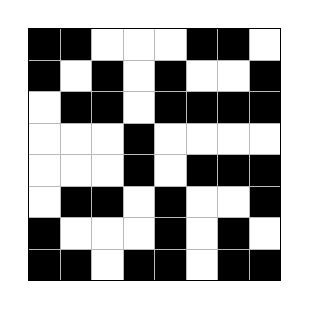
\begin{tikzpicture}[scale=0.4]
  \fill[black] (0,0) rectangle ++(1,-1);
  \fill[black] (1,0) rectangle ++(1,-1);
  \fill[black] (5,0) rectangle ++(1,-1);
  \fill[black] (6,0) rectangle ++(1,-1);
  \fill[black] (0,-1) rectangle ++(1,-1);
  \fill[black] (2,-1) rectangle ++(1,-1);
  \fill[black] (4,-1) rectangle ++(1,-1);
  \fill[black] (7,-1) rectangle ++(1,-1);
  \fill[black] (1,-2) rectangle ++(1,-1);
  \fill[black] (2,-2) rectangle ++(1,-1);
  \fill[black] (4,-2) rectangle ++(1,-1);
  \fill[black] (5,-2) rectangle ++(1,-1);
  \fill[black] (6,-2) rectangle ++(1,-1);
  \fill[black] (7,-2) rectangle ++(1,-1);
  \fill[black] (3,-3) rectangle ++(1,-1);
  \fill[black] (3,-4) rectangle ++(1,-1);
  \fill[black] (5,-4) rectangle ++(1,-1);
  \fill[black] (6,-4) rectangle ++(1,-1);
  \fill[black] (7,-4) rectangle ++(1,-1);
  \fill[black] (1,-5) rectangle ++(1,-1);
  \fill[black] (2,-5) rectangle ++(1,-1);
  \fill[black] (4,-5) rectangle ++(1,-1);
  \fill[black] (7,-5) rectangle ++(1,-1);
  \fill[black] (0,-6) rectangle ++(1,-1);
  \fill[black] (4,-6) rectangle ++(1,-1);
  \fill[black] (6,-6) rectangle ++(1,-1);
  \fill[black] (0,-7) rectangle ++(1,-1);
  \fill[black] (1,-7) rectangle ++(1,-1);
  \fill[black] (3,-7) rectangle ++(1,-1);
  \fill[black] (4,-7) rectangle ++(1,-1);
  \fill[black] (6,-7) rectangle ++(1,-1);
  \fill[black] (7,-7) rectangle ++(1,-1);
  \draw[step=1,gray!55,line width=0.15pt] (0,-8) grid (8,0);
  \draw[black,line width=0.5pt] (0,-8) rectangle (8,0);
  \end{tikzpicture}
  \\[3pt]{\small (a) $n=8$, $32$ cells (proven)}
  \end{minipage}\hfill
  \begin{minipage}[b]{0.3\textwidth}\centering
  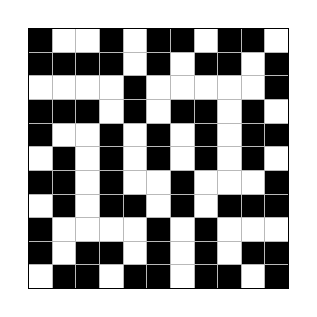
\begin{tikzpicture}[scale=0.3]
  \fill[black] (0,0) rectangle ++(1,-1);
  \fill[black] (3,0) rectangle ++(1,-1);
  \fill[black] (5,0) rectangle ++(1,-1);
  \fill[black] (6,0) rectangle ++(1,-1);
  \fill[black] (8,0) rectangle ++(1,-1);
  \fill[black] (9,0) rectangle ++(1,-1);
  \fill[black] (0,-1) rectangle ++(1,-1);
  \fill[black] (1,-1) rectangle ++(1,-1);
  \fill[black] (2,-1) rectangle ++(1,-1);
  \fill[black] (3,-1) rectangle ++(1,-1);
  \fill[black] (5,-1) rectangle ++(1,-1);
  \fill[black] (7,-1) rectangle ++(1,-1);
  \fill[black] (8,-1) rectangle ++(1,-1);
  \fill[black] (10,-1) rectangle ++(1,-1);
  \fill[black] (4,-2) rectangle ++(1,-1);
  \fill[black] (10,-2) rectangle ++(1,-1);
  \fill[black] (0,-3) rectangle ++(1,-1);
  \fill[black] (1,-3) rectangle ++(1,-1);
  \fill[black] (2,-3) rectangle ++(1,-1);
  \fill[black] (4,-3) rectangle ++(1,-1);
  \fill[black] (6,-3) rectangle ++(1,-1);
  \fill[black] (7,-3) rectangle ++(1,-1);
  \fill[black] (9,-3) rectangle ++(1,-1);
  \fill[black] (0,-4) rectangle ++(1,-1);
  \fill[black] (3,-4) rectangle ++(1,-1);
  \fill[black] (5,-4) rectangle ++(1,-1);
  \fill[black] (7,-4) rectangle ++(1,-1);
  \fill[black] (9,-4) rectangle ++(1,-1);
  \fill[black] (10,-4) rectangle ++(1,-1);
  \fill[black] (1,-5) rectangle ++(1,-1);
  \fill[black] (3,-5) rectangle ++(1,-1);
  \fill[black] (5,-5) rectangle ++(1,-1);
  \fill[black] (7,-5) rectangle ++(1,-1);
  \fill[black] (9,-5) rectangle ++(1,-1);
  \fill[black] (0,-6) rectangle ++(1,-1);
  \fill[black] (1,-6) rectangle ++(1,-1);
  \fill[black] (3,-6) rectangle ++(1,-1);
  \fill[black] (6,-6) rectangle ++(1,-1);
  \fill[black] (10,-6) rectangle ++(1,-1);
  \fill[black] (1,-7) rectangle ++(1,-1);
  \fill[black] (3,-7) rectangle ++(1,-1);
  \fill[black] (4,-7) rectangle ++(1,-1);
  \fill[black] (6,-7) rectangle ++(1,-1);
  \fill[black] (8,-7) rectangle ++(1,-1);
  \fill[black] (9,-7) rectangle ++(1,-1);
  \fill[black] (10,-7) rectangle ++(1,-1);
  \fill[black] (0,-8) rectangle ++(1,-1);
  \fill[black] (5,-8) rectangle ++(1,-1);
  \fill[black] (7,-8) rectangle ++(1,-1);
  \fill[black] (0,-9) rectangle ++(1,-1);
  \fill[black] (2,-9) rectangle ++(1,-1);
  \fill[black] (3,-9) rectangle ++(1,-1);
  \fill[black] (5,-9) rectangle ++(1,-1);
  \fill[black] (7,-9) rectangle ++(1,-1);
  \fill[black] (9,-9) rectangle ++(1,-1);
  \fill[black] (10,-9) rectangle ++(1,-1);
  \fill[black] (1,-10) rectangle ++(1,-1);
  \fill[black] (2,-10) rectangle ++(1,-1);
  \fill[black] (4,-10) rectangle ++(1,-1);
  \fill[black] (5,-10) rectangle ++(1,-1);
  \fill[black] (7,-10) rectangle ++(1,-1);
  \fill[black] (8,-10) rectangle ++(1,-1);
  \fill[black] (10,-10) rectangle ++(1,-1);
  \draw[step=1,gray!55,line width=0.15pt] (0,-11) grid (11,0);
  \draw[black,line width=0.5pt] (0,-11) rectangle (11,0);
  \end{tikzpicture}
  \\[3pt]{\small (b) $n=11$, $63$ cells (proven)}
  \end{minipage}\hfill
  \begin{minipage}[b]{0.36\textwidth}\centering
  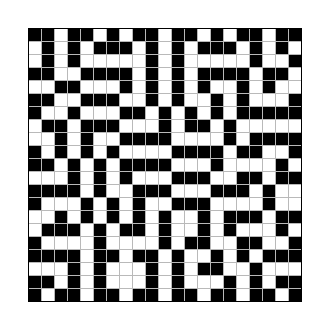
\begin{tikzpicture}[scale=0.165]
  \fill[black] (0,0) rectangle ++(1,-1);
  \fill[black] (1,0) rectangle ++(1,-1);
  \fill[black] (3,0) rectangle ++(1,-1);
  \fill[black] (4,0) rectangle ++(1,-1);
  \fill[black] (6,0) rectangle ++(1,-1);
  \fill[black] (8,0) rectangle ++(1,-1);
  \fill[black] (9,0) rectangle ++(1,-1);
  \fill[black] (11,0) rectangle ++(1,-1);
  \fill[black] (12,0) rectangle ++(1,-1);
  \fill[black] (14,0) rectangle ++(1,-1);
  \fill[black] (16,0) rectangle ++(1,-1);
  \fill[black] (17,0) rectangle ++(1,-1);
  \fill[black] (19,0) rectangle ++(1,-1);
  \fill[black] (20,0) rectangle ++(1,-1);
  \fill[black] (1,-1) rectangle ++(1,-1);
  \fill[black] (3,-1) rectangle ++(1,-1);
  \fill[black] (5,-1) rectangle ++(1,-1);
  \fill[black] (6,-1) rectangle ++(1,-1);
  \fill[black] (7,-1) rectangle ++(1,-1);
  \fill[black] (9,-1) rectangle ++(1,-1);
  \fill[black] (11,-1) rectangle ++(1,-1);
  \fill[black] (13,-1) rectangle ++(1,-1);
  \fill[black] (14,-1) rectangle ++(1,-1);
  \fill[black] (15,-1) rectangle ++(1,-1);
  \fill[black] (17,-1) rectangle ++(1,-1);
  \fill[black] (19,-1) rectangle ++(1,-1);
  \fill[black] (1,-2) rectangle ++(1,-1);
  \fill[black] (3,-2) rectangle ++(1,-1);
  \fill[black] (9,-2) rectangle ++(1,-1);
  \fill[black] (11,-2) rectangle ++(1,-1);
  \fill[black] (17,-2) rectangle ++(1,-1);
  \fill[black] (20,-2) rectangle ++(1,-1);
  \fill[black] (0,-3) rectangle ++(1,-1);
  \fill[black] (1,-3) rectangle ++(1,-1);
  \fill[black] (4,-3) rectangle ++(1,-1);
  \fill[black] (5,-3) rectangle ++(1,-1);
  \fill[black] (6,-3) rectangle ++(1,-1);
  \fill[black] (7,-3) rectangle ++(1,-1);
  \fill[black] (9,-3) rectangle ++(1,-1);
  \fill[black] (11,-3) rectangle ++(1,-1);
  \fill[black] (13,-3) rectangle ++(1,-1);
  \fill[black] (14,-3) rectangle ++(1,-1);
  \fill[black] (15,-3) rectangle ++(1,-1);
  \fill[black] (16,-3) rectangle ++(1,-1);
  \fill[black] (18,-3) rectangle ++(1,-1);
  \fill[black] (19,-3) rectangle ++(1,-1);
  \fill[black] (2,-4) rectangle ++(1,-1);
  \fill[black] (3,-4) rectangle ++(1,-1);
  \fill[black] (7,-4) rectangle ++(1,-1);
  \fill[black] (9,-4) rectangle ++(1,-1);
  \fill[black] (11,-4) rectangle ++(1,-1);
  \fill[black] (13,-4) rectangle ++(1,-1);
  \fill[black] (16,-4) rectangle ++(1,-1);
  \fill[black] (18,-4) rectangle ++(1,-1);
  \fill[black] (0,-5) rectangle ++(1,-1);
  \fill[black] (1,-5) rectangle ++(1,-1);
  \fill[black] (4,-5) rectangle ++(1,-1);
  \fill[black] (5,-5) rectangle ++(1,-1);
  \fill[black] (6,-5) rectangle ++(1,-1);
  \fill[black] (9,-5) rectangle ++(1,-1);
  \fill[black] (11,-5) rectangle ++(1,-1);
  \fill[black] (14,-5) rectangle ++(1,-1);
  \fill[black] (16,-5) rectangle ++(1,-1);
  \fill[black] (20,-5) rectangle ++(1,-1);
  \fill[black] (0,-6) rectangle ++(1,-1);
  \fill[black] (3,-6) rectangle ++(1,-1);
  \fill[black] (7,-6) rectangle ++(1,-1);
  \fill[black] (8,-6) rectangle ++(1,-1);
  \fill[black] (10,-6) rectangle ++(1,-1);
  \fill[black] (12,-6) rectangle ++(1,-1);
  \fill[black] (14,-6) rectangle ++(1,-1);
  \fill[black] (16,-6) rectangle ++(1,-1);
  \fill[black] (17,-6) rectangle ++(1,-1);
  \fill[black] (18,-6) rectangle ++(1,-1);
  \fill[black] (19,-6) rectangle ++(1,-1);
  \fill[black] (20,-6) rectangle ++(1,-1);
  \fill[black] (1,-7) rectangle ++(1,-1);
  \fill[black] (2,-7) rectangle ++(1,-1);
  \fill[black] (4,-7) rectangle ++(1,-1);
  \fill[black] (5,-7) rectangle ++(1,-1);
  \fill[black] (6,-7) rectangle ++(1,-1);
  \fill[black] (10,-7) rectangle ++(1,-1);
  \fill[black] (12,-7) rectangle ++(1,-1);
  \fill[black] (13,-7) rectangle ++(1,-1);
  \fill[black] (15,-7) rectangle ++(1,-1);
  \fill[black] (2,-8) rectangle ++(1,-1);
  \fill[black] (4,-8) rectangle ++(1,-1);
  \fill[black] (7,-8) rectangle ++(1,-1);
  \fill[black] (8,-8) rectangle ++(1,-1);
  \fill[black] (9,-8) rectangle ++(1,-1);
  \fill[black] (10,-8) rectangle ++(1,-1);
  \fill[black] (15,-8) rectangle ++(1,-1);
  \fill[black] (17,-8) rectangle ++(1,-1);
  \fill[black] (18,-8) rectangle ++(1,-1);
  \fill[black] (19,-8) rectangle ++(1,-1);
  \fill[black] (20,-8) rectangle ++(1,-1);
  \fill[black] (0,-9) rectangle ++(1,-1);
  \fill[black] (2,-9) rectangle ++(1,-1);
  \fill[black] (4,-9) rectangle ++(1,-1);
  \fill[black] (6,-9) rectangle ++(1,-1);
  \fill[black] (11,-9) rectangle ++(1,-1);
  \fill[black] (12,-9) rectangle ++(1,-1);
  \fill[black] (13,-9) rectangle ++(1,-1);
  \fill[black] (14,-9) rectangle ++(1,-1);
  \fill[black] (16,-9) rectangle ++(1,-1);
  \fill[black] (17,-9) rectangle ++(1,-1);
  \fill[black] (20,-9) rectangle ++(1,-1);
  \fill[black] (0,-10) rectangle ++(1,-1);
  \fill[black] (1,-10) rectangle ++(1,-1);
  \fill[black] (3,-10) rectangle ++(1,-1);
  \fill[black] (5,-10) rectangle ++(1,-1);
  \fill[black] (7,-10) rectangle ++(1,-1);
  \fill[black] (8,-10) rectangle ++(1,-1);
  \fill[black] (9,-10) rectangle ++(1,-1);
  \fill[black] (10,-10) rectangle ++(1,-1);
  \fill[black] (14,-10) rectangle ++(1,-1);
  \fill[black] (19,-10) rectangle ++(1,-1);
  \fill[black] (3,-11) rectangle ++(1,-1);
  \fill[black] (5,-11) rectangle ++(1,-1);
  \fill[black] (7,-11) rectangle ++(1,-1);
  \fill[black] (11,-11) rectangle ++(1,-1);
  \fill[black] (12,-11) rectangle ++(1,-1);
  \fill[black] (13,-11) rectangle ++(1,-1);
  \fill[black] (16,-11) rectangle ++(1,-1);
  \fill[black] (17,-11) rectangle ++(1,-1);
  \fill[black] (19,-11) rectangle ++(1,-1);
  \fill[black] (20,-11) rectangle ++(1,-1);
  \fill[black] (0,-12) rectangle ++(1,-1);
  \fill[black] (1,-12) rectangle ++(1,-1);
  \fill[black] (2,-12) rectangle ++(1,-1);
  \fill[black] (3,-12) rectangle ++(1,-1);
  \fill[black] (5,-12) rectangle ++(1,-1);
  \fill[black] (8,-12) rectangle ++(1,-1);
  \fill[black] (9,-12) rectangle ++(1,-1);
  \fill[black] (10,-12) rectangle ++(1,-1);
  \fill[black] (14,-12) rectangle ++(1,-1);
  \fill[black] (15,-12) rectangle ++(1,-1);
  \fill[black] (16,-12) rectangle ++(1,-1);
  \fill[black] (18,-12) rectangle ++(1,-1);
  \fill[black] (0,-13) rectangle ++(1,-1);
  \fill[black] (4,-13) rectangle ++(1,-1);
  \fill[black] (6,-13) rectangle ++(1,-1);
  \fill[black] (8,-13) rectangle ++(1,-1);
  \fill[black] (11,-13) rectangle ++(1,-1);
  \fill[black] (12,-13) rectangle ++(1,-1);
  \fill[black] (13,-13) rectangle ++(1,-1);
  \fill[black] (18,-13) rectangle ++(1,-1);
  \fill[black] (2,-14) rectangle ++(1,-1);
  \fill[black] (4,-14) rectangle ++(1,-1);
  \fill[black] (6,-14) rectangle ++(1,-1);
  \fill[black] (8,-14) rectangle ++(1,-1);
  \fill[black] (10,-14) rectangle ++(1,-1);
  \fill[black] (13,-14) rectangle ++(1,-1);
  \fill[black] (15,-14) rectangle ++(1,-1);
  \fill[black] (16,-14) rectangle ++(1,-1);
  \fill[black] (17,-14) rectangle ++(1,-1);
  \fill[black] (19,-14) rectangle ++(1,-1);
  \fill[black] (20,-14) rectangle ++(1,-1);
  \fill[black] (1,-15) rectangle ++(1,-1);
  \fill[black] (2,-15) rectangle ++(1,-1);
  \fill[black] (3,-15) rectangle ++(1,-1);
  \fill[black] (5,-15) rectangle ++(1,-1);
  \fill[black] (7,-15) rectangle ++(1,-1);
  \fill[black] (8,-15) rectangle ++(1,-1);
  \fill[black] (10,-15) rectangle ++(1,-1);
  \fill[black] (13,-15) rectangle ++(1,-1);
  \fill[black] (15,-15) rectangle ++(1,-1);
  \fill[black] (19,-15) rectangle ++(1,-1);
  \fill[black] (0,-16) rectangle ++(1,-1);
  \fill[black] (5,-16) rectangle ++(1,-1);
  \fill[black] (10,-16) rectangle ++(1,-1);
  \fill[black] (12,-16) rectangle ++(1,-1);
  \fill[black] (13,-16) rectangle ++(1,-1);
  \fill[black] (16,-16) rectangle ++(1,-1);
  \fill[black] (17,-16) rectangle ++(1,-1);
  \fill[black] (20,-16) rectangle ++(1,-1);
  \fill[black] (0,-17) rectangle ++(1,-1);
  \fill[black] (1,-17) rectangle ++(1,-1);
  \fill[black] (2,-17) rectangle ++(1,-1);
  \fill[black] (3,-17) rectangle ++(1,-1);
  \fill[black] (5,-17) rectangle ++(1,-1);
  \fill[black] (6,-17) rectangle ++(1,-1);
  \fill[black] (8,-17) rectangle ++(1,-1);
  \fill[black] (9,-17) rectangle ++(1,-1);
  \fill[black] (11,-17) rectangle ++(1,-1);
  \fill[black] (14,-17) rectangle ++(1,-1);
  \fill[black] (16,-17) rectangle ++(1,-1);
  \fill[black] (18,-17) rectangle ++(1,-1);
  \fill[black] (19,-17) rectangle ++(1,-1);
  \fill[black] (20,-17) rectangle ++(1,-1);
  \fill[black] (3,-18) rectangle ++(1,-1);
  \fill[black] (5,-18) rectangle ++(1,-1);
  \fill[black] (9,-18) rectangle ++(1,-1);
  \fill[black] (11,-18) rectangle ++(1,-1);
  \fill[black] (13,-18) rectangle ++(1,-1);
  \fill[black] (14,-18) rectangle ++(1,-1);
  \fill[black] (17,-18) rectangle ++(1,-1);
  \fill[black] (0,-19) rectangle ++(1,-1);
  \fill[black] (1,-19) rectangle ++(1,-1);
  \fill[black] (3,-19) rectangle ++(1,-1);
  \fill[black] (5,-19) rectangle ++(1,-1);
  \fill[black] (9,-19) rectangle ++(1,-1);
  \fill[black] (11,-19) rectangle ++(1,-1);
  \fill[black] (15,-19) rectangle ++(1,-1);
  \fill[black] (17,-19) rectangle ++(1,-1);
  \fill[black] (19,-19) rectangle ++(1,-1);
  \fill[black] (20,-19) rectangle ++(1,-1);
  \fill[black] (0,-20) rectangle ++(1,-1);
  \fill[black] (2,-20) rectangle ++(1,-1);
  \fill[black] (3,-20) rectangle ++(1,-1);
  \fill[black] (5,-20) rectangle ++(1,-1);
  \fill[black] (6,-20) rectangle ++(1,-1);
  \fill[black] (8,-20) rectangle ++(1,-1);
  \fill[black] (9,-20) rectangle ++(1,-1);
  \fill[black] (11,-20) rectangle ++(1,-1);
  \fill[black] (12,-20) rectangle ++(1,-1);
  \fill[black] (14,-20) rectangle ++(1,-1);
  \fill[black] (15,-20) rectangle ++(1,-1);
  \fill[black] (17,-20) rectangle ++(1,-1);
  \fill[black] (18,-20) rectangle ++(1,-1);
  \fill[black] (20,-20) rectangle ++(1,-1);
  \draw[step=1,gray!55,line width=0.15pt] (0,-21) grid (21,0);
  \draw[black,line width=0.5pt] (0,-21) rectangle (21,0);
  \end{tikzpicture}
  \\[3pt]{\small (c) $n=21$, $221$ cells (best-found)}
  \end{minipage}
  \caption{Representative verifier-validated connected still lifes. (a,b) proven connected optima at $n=8$ and $n=11$; (c) a best-found pattern at $n=21$. Filled squares are live cells; in every panel the pattern is stable, induces no birth in the box or its one-cell exterior ring, and forms a single $8$-connected component. The $n=8$ and $n=11$ panels are the witnesses underlying the proven entries of Table~\ref{tab:main}; all three pass the released verifier in the official submission format.}
  \label{fig:witness}
\end{figure}

\section{Limitations}
\label{sec:limitations}
Our proven results stop at $n=11$; for $n=13$ and $n=15$ we report bounded best-found values, and for $16\le n\le 21$ best-found patterns whose gap to the ceiling we do not claim to have closed. Exact proof at larger $n$ was limited by the hardness of connectivity-constrained search on a single passively-cooled laptop within a fixed time budget, not by any closed-form barrier. Our naive simulated-annealing proposer did not produce valid moves and we did not have time to implement the structured-neighborhood or large-neighborhood-repair variants that Section~\ref{sec:sa} argues are needed; consequently the large-$n$ entries are weaker than the small-$n$ ones. The optimality of $n=10$ and $n=11$ is supported by two structurally independent connectivity encodings within CP-SAT (flow and spanning tree) that agree on the optimum from different witnesses, which eliminates a connectivity-modeling error; a fully solver-independent confirmation remains partial, since our ASP stability-only enumeration at the ceiling found only disconnected configurations but did not exhaust the space for these two boxes within budget. We judge the residual risk low, but a terminating non-CP-SAT optimality proof for $n=10,11$ would close the gap entirely. We did not attempt $n=31$ or $n=32$ within budget and exclude them from our reported results. Finally, all upper bounds inherit the correctness of the published unconstrained optima~\citep{chu2012}.

\section{Conclusion}
\label{sec:conclusion}
We presented a verifier-grounded agentic loop and used it to produce, to our knowledge, the first per-$n$ table of connected maximum-density still lifes for the small boxes, with proven optima for $n\in\{8,9,10,11\}$ and bounded best-found values beyond. The methodological yield---the ceiling-matching proof rule, the comparison of flow, spanning-tree, and reachability connectivity encodings, and the diagnosis of why naive local search fails---is, for an AI-for-science venue, as much the point as the patterns. We release the verifier, both CP-SAT connectivity encodings, the corrected ASP encoding, and all witness artifacts so that every reported value is independently machine-checkable.

\begin{ack}
% This section is automatically hidden in the anonymized submission and appears
% only in the camera-ready [final] build. Add funding and competing-interests
% disclosures here for camera-ready. [T6]
\end{ack}

% ----------------------------------------------------------------------------
\section*{References}
\small
\begin{thebibliography}{99}

\bibitem{chu2012}
G.~Chu and P.~J.~Stuckey.
A complete solution to the maximum density still life problem.
\emph{Artificial Intelligence}, 184--185:1--16, 2012.

\bibitem{oeis}
OEIS Foundation Inc.
Sequence A055397: Maximum population of an $n\times n$ stable pattern in Conway's Game of Life.
\emph{The On-Line Encyclopedia of Integer Sequences}.

\bibitem{elkies1998}
N.~D.~Elkies.
The still-life density problem and its generalizations.
arXiv:math/9905194, 1998.

\bibitem{bosch2004}
R.~Bosch and M.~Trick.
Constraint programming and hybrid formulations for three Life designs.
\emph{Annals of Operations Research}, 130:41--56, 2004.

\bibitem{larrosa2005}
J.~Larrosa, E.~Morancho, and D.~Niso.
On the practical use of variable elimination in constraint optimization problems: `still-life' as a case study.
\emph{Journal of Artificial Intelligence Research}, 23:421--440, 2005.

\bibitem{chu2010}
G.~Chu, K.~E.~Petrie, and N.~Yorke-Smith.
Constraint programming to solve maximal density still life.
In \emph{Game of Life Cellular Automata}, chapter 10, pages 99--114. Springer, 2010.

\bibitem{gallardo2009}
J.~E.~Gallardo, C.~Cotta, and A.~J.~Fern\'andez.
Finding still lifes with memetic/exact hybrid algorithms.
arXiv:0812.4170, 2008.

\bibitem{aspcomp2013}
M.~Alviano et al.
The Fourth Answer Set Programming Competition: Preliminary report.
In \emph{Logic Programming and Nonmonotonic Reasoning (LPNMR 2013)}, LNCS 8148, pages 42--53. Springer, 2013.
Connected Maximum-Density Still Life benchmark; Official Problem Suite, \url{https://www.mat.unical.it/aspcomp2013/}.

\bibitem{funsearch}
B.~Romera-Paredes et al.
Mathematical discoveries from program search with large language models.
\emph{Nature}, 625:468--475, 2024.

\bibitem{alphaevolve}
A.~Novikov et al.
AlphaEvolve: A coding agent for scientific and algorithmic discovery.
arXiv:2506.13131, 2025.

\bibitem{satlution}
C.~Yu, R.~Liang, C.-T.~Ho, and H.~Ren.
Autonomous code evolution meets NP-completeness.
arXiv:2509.07367, 2025.

\bibitem{problem}
Curated by Siddhartha Mahajan (2026).
Connected Still Life.
Reviewed by Dr.\ Ankan Pal.
CAISc 2026 Verifiable Problems Track.
\url{https://caisc2026.github.io/verifiable-problems/?problem=connected-still-life}.

\end{thebibliography}

\newpage

% ============================================================================
\section*{Conference For AI Scientists 2026 - AI Involvement Checklist}
\label{checklist_ai_involvement}

% Instruction block deleted per template directions; section/subsection headings,
% questions, answers, and guidelines retained.

\subsection*{Research Stage Assessment}

For items 1-4, give a score from the scale below that defines the role of AI in each part of the scientific process. The scores are as follows:

\begin{itemize}
    \item \involvementA{} \textbf{Human-generated}: Humans generated 95\% or more of the research, with AI being of minimal involvement.
    \item \involvementB{} \textbf{Mostly human, assisted by AI}: The research was a collaboration between humans and AI models, but humans produced the majority (>50\%) of the research.
    \item \involvementC{} \textbf{Mostly AI, assisted by human}: The research task was a collaboration between humans and AI models, but AI produced the majority (>50\%) of the research.
    \item \involvementD{} \textbf{AI-generated}: AI performed over 95\% of the research. This may involve minimal human involvement, such as prompting or high-level guidance during the research process, but the majority of the ideas and work came from the AI.
\end{itemize}

For each research stage where AI was involved, please also indicate the approximate level of iteration effort using the provided iteration macros. Count substantive attempts, prompts, runs, agent trajectories, or course corrections; do not count minor wording edits.

\begin{itemize}
    \item \iterationLow{}: approximately 1-10 substantive attempts.
    \item \iterationMedium{}: approximately 10-100 substantive attempts, with some failed attempts or course corrections.
    \item \iterationHigh{}: approximately 100+ substantive attempts, with substantial exploration, failures, or trial-and-error.
    \item \iterationNA{}: not applicable because AI involvement was \involvementA{}.
    \item \iterationUnclear{}: the authors cannot reasonably estimate.
\end{itemize}

% [T7 DONE] AI Involvement grades confirmed by the author.
\begin{enumerate}

    \item \textbf{Hypothesis development}.

    Answer: \involvementC{}

    Iteration Effort: \iterationMedium{}

    Explanation: The human author selected the venue and the verifiable track and steered the topic toward the connected variant. A large language model then conducted the background literature search that established the absence of any published per-$n$ connected-optima table, framed the gap, and proposed the verifier--proposer methodology. Idea generation and the supporting research were thus majority-AI, with human direction setting scope and goals.

    \item \textbf{Experimental design and implementation}.

    Answer: \involvementC{}

    Iteration Effort: \iterationHigh{}

    Explanation: An agentic coding assistant wrote the verifier, the CP-SAT flow model, the reproduced ASP encoding, and the experiment harness, and executed all runs. The human made the consequential strategic decisions (choice of connectivity encoding, sweep ordering, stopping criteria, and the decision to cross-check). Iteration was high: encoding bugs, a solver-API misreading, core oversubscription crashes, and a failed simulated-annealing design were diagnosed and corrected over many runs.

    \item \textbf{Analysis of data and interpretation of results}.

    Answer: \involvementC{}

    Iteration Effort: \iterationMedium{}

    Explanation: The AI organized run logs, derived the ceiling-matching argument, computed the connectivity penalties and bounds, and produced the solver comparison and the diagnosis of the simulated-annealing failure. The human reviewed and validated interpretations, particularly the soundness of the optimality claims and the honesty of the labeling.

    \item \textbf{Writing}.

    Answer: \involvementC{}

    Iteration Effort: \iterationMedium{}

    Explanation: The manuscript text, tables, and narrative were drafted by a large language model from the experiment log and were revised under human direction and review. The human set the framing priorities, checked all claims against the verified results, and is responsible for the final content.

\end{enumerate}

\subsection*{AI System Documentation}

\begin{enumerate}
    \setcounter{enumi}{4}

    \item \textbf{AI systems used}.

    Description: A single frontier large language model was used in three roles: (i) conversational research and ideation; (ii) an agentic coding assistant with file-system and code-execution access that engineered the verifier, the exact engines, and the experiment harness and ran all experiments; and (iii) manuscript drafting. The exact solving used a standard off-the-shelf CP-SAT constraint solver and a standard answer-set-programming solver, both invoked by the agent; these are conventional combinatorial tools, not AI systems. Specific product and model names are omitted here per the submission guidelines and will be provided in the camera-ready version.

    \item \textbf{Observed AI Limitations}.

    Description: We observed several concrete failure modes. The model reproduced a constraint encoding with a silent semantic error (an aggregate that failed to count neighbors), which produced no valid solutions and was detected only by the independent verifier. It initially misread a solver's optimality signal, briefly mislabeling a proven result as unproven. It oversubscribed CPU cores in a way that crashed the solver on the target hardware. And its first simulated-annealing design made no valid moves on a tightly constrained problem, requiring a redesign that time did not permit. In each case the deterministic verifier or an internal consistency check, rather than the model's own confidence, surfaced the error---reinforcing the value of grounding generative components in an exact checker.

\end{enumerate}

\newpage

% ============================================================================
\section*{Conference For AI Scientists 2026 - Reproducibility and Responsibility Checklist}
\label{checklist_reproducibility}

% Instruction block deleted per template directions; section headings, questions,
% answers, and guidelines retained.

\begin{enumerate}

\item {\bf Claims}
    \item[] Question: Do the main claims made in the abstract and introduction accurately reflect the paper's contributions and scope?
    \item[] Answer: \answerYes{}
    \item[] Justification: The abstract and Section~\ref{sec:intro} state proven optimality only for $n\in\{8,9,10,11\}$ and label all other values best-found with bounds, matching Table~\ref{tab:main}.
    \item[] Guidelines:
    \begin{itemize}
        \item The answer NA means that the abstract and introduction do not include the claims made in the paper.
        \item The abstract and/or introduction should clearly state the claims made, including the contributions made in the paper and important assumptions and limitations. A No or NA answer to this question will not be perceived well by the reviewers.
        \item The claims made should match theoretical and experimental results, and reflect how much the results can be expected to generalize to other settings.
        \item It is fine to include aspirational goals as motivation as long as it is clear that these goals are not attained by the paper.
    \end{itemize}

\item {\bf Limitations}
    \item[] Question: Does the paper discuss the limitations of the work performed by the authors?
    \item[] Answer: \answerYes{}
    \item[] Justification: Section~\ref{sec:limitations} discusses the proof horizon at $n=11$, the unclosed gaps for $n\ge 13$, the simulated-annealing failure, the single-effort implementation risk, and the dependence on published unconstrained optima.
    \item[] Guidelines:
    \begin{itemize}
        \item The answer NA means that the paper has no limitation while the answer No means that the paper has limitations, but those are not discussed in the paper.
        \item The authors are encouraged to create a separate "Limitations" section in their paper.
        \item The paper should point out any strong assumptions and how robust the results are to violations of these assumptions.
        \item The authors should reflect on the scope of the claims made and the factors that influence performance.
        \item The authors should discuss the computational efficiency of the proposed algorithms and how they scale.
        \item Reviewers will be instructed to not penalize honesty concerning limitations.
    \end{itemize}

\item {\bf Theory assumptions and proofs}
    \item[] Question: For each theoretical result, does the paper provide the full set of assumptions and a complete (and correct) proof?
    \item[] Answer: \answerYes{}
    \item[] Justification: Proposition~\ref{prop:ceiling} is stated with its assumptions (correctness of the published unconstrained optima and of the verifier) and proved; the remaining optimality results are computational (exhaustive search), cross-checked between two independent solvers.
    \item[] Guidelines:
    \begin{itemize}
        \item The answer NA means that the paper does not include theoretical results.
        \item All theorems, formulas, and proofs should be numbered and cross-referenced.
        \item All assumptions should be clearly stated or referenced in the statement of any theorems.
        \item Proofs can appear in the main paper or supplemental material with a proof sketch for intuition.
    \end{itemize}

    \item {\bf Experimental result reproducibility}
    \item[] Question: Does the paper fully disclose all the information needed to reproduce the main experimental results?
    \item[] Answer: \answerYes{}
    \item[] Justification: We give the exact encodings (flow connectivity and the corrected ASP program), solver versions, random seeds, thread counts, and per-$n$ time budgets, and release the verifier and all witness JSONs in the submission format.
    \item[] Guidelines:
    \begin{itemize}
        \item The answer NA means that the paper does not include experiments.
        \item A No answer will not be perceived well: making the paper reproducible is important.
        \item Authors should describe steps taken to make results reproducible or verifiable.
        \item Authors are welcome to describe the particular way they provide for reproducibility.
    \end{itemize}

\item {\bf Open access to data and code}
    \item[] Question: Does the paper provide open access to the data and code, with sufficient instructions to faithfully reproduce the main experimental results?
    \item[] Answer: \answerYes{}
    \item[] Justification: The verifier, the solver encodings, and every witness pattern are released (anonymized) as supplementary material with run instructions; the witnesses are in the official machine-checkable format.
    \item[] Guidelines:
    \begin{itemize}
        \item The answer NA means that the paper does not include experiments requiring code.
        \item ``No'' is acceptable, but releasing code and data is encouraged.
        \item At submission time, anonymized versions should be released to preserve anonymity.
        \item Instructions should contain the exact command and environment needed to reproduce the results.
    \end{itemize}

\item {\bf Experimental setting/details}
    \item[] Question: Does the paper specify all the training and test details necessary to understand the results?
    \item[] Answer: \answerYes{}
    \item[] Justification: Sections~\ref{sec:method}--\ref{sec:results} and Table~\ref{tab:main} specify the encodings, the objective, solver seeds and thread counts, and the time budgets per box.
    \item[] Guidelines:
    \begin{itemize}
        \item The answer NA means that the paper does not include experiments.
        \item The experimental setting should be presented to a level of detail necessary to appreciate the results.
        \item Full details can be provided with the code, in an appendix, or as supplemental material.
    \end{itemize}

\item {\bf Experiment statistical significance}
    \item[] Question: Does the paper report error bars suitably and correctly defined or other appropriate information about the statistical significance of the experiments?
    \item[] Answer: \answerNA{}
    \item[] Justification: The primary results are exact, deterministic, verifier-checked combinatorial facts (proven optima and validated witnesses), not statistical estimates, so error bars do not apply; for the stochastic proposer we report the best verified result over documented seeds.
    \item[] Guidelines:
    \begin{itemize}
        \item The answer NA means that the paper does not include experiments.
        \item Authors should answer ``Yes'' if results are accompanied by error bars, confidence intervals, or significance tests.
        \item The factors of variability captured by the error bars should be clearly stated.
    \end{itemize}

\item {\bf Experiments compute resources}
    \item[] Question: For each experiment, does the paper provide sufficient information on the computer resources needed to reproduce the experiments?
    \item[] Answer: \answerYes{}
    \item[] Justification: All experiments ran on a single fanless laptop using four performance cores and 24~GB of unified memory; per-$n$ wall-clock times are reported, and total compute is modest (minutes per proven box).
    \item[] Guidelines:
    \begin{itemize}
        \item The answer NA means that the paper does not include experiments.
        \item The paper should indicate the type of compute workers, memory, and storage.
        \item The paper should provide per-run and total compute estimates.
    \end{itemize}

\item {\bf Research Ethics}
    \item[] Question: Does the research conducted in the paper conform with the NeurIPS Code of Ethics, except where CAISc's AI authorship policies apply?
    \item[] Answer: \answerYes{}
    \item[] Justification: The work is purely combinatorial, involves no human subjects or personal data, and follows the Code of Ethics; the only deviation is the conference's own AI-authorship policy, which we follow as specified.
    \item[] Guidelines:
    \begin{itemize}
        \item All submissions should adhere to the NeurIPS Code of Ethics, except where CAISc's AI authorship policies apply.
        \item The answer NA means the authors have not reviewed the Code of Ethics.
        \item If the authors answer No, they should explain the special circumstances.
    \end{itemize}

\item {\bf Broader impacts}
    \item[] Question: Does the paper discuss both potential positive societal impacts and negative societal impacts of the work performed?
    \item[] Answer: \answerYes{}
    \item[] Justification: Positive impacts include a reproducible, verifier-grounded template for AI-assisted combinatorial discovery; potential negative impacts are limited to the general dual-use nature of stronger automated optimization and agentic tooling, mitigated here by the emphasis on machine-checkable artifacts.
    \item[] Guidelines:
    \begin{itemize}
        \item The answer NA means that there is no societal impact of the work performed.
        \item If the authors answer NA or No, they should explain why.
        \item Examples of negative impacts include malicious or unintended uses, fairness, privacy, and security considerations.
        \item If there are negative impacts, authors could discuss mitigation strategies.
    \end{itemize}

\end{enumerate}

\end{document}
